\section{Experimental methods}\label{supp:fields}\label{supp:metrics}
\subsection{Network, path sets, and demand settings}\label{supp:networks}
The public Sioux Falls network has $24$ nodes and $76$ directed arcs
\citep{tnfrc2024transportation}. All arcs belong to one cycle atom, hence
one compatibility class. The eight queries are the positive-demand OD pairs with the largest
published demands, with ties broken by ascending origin then destination
node ID. All happen to involve node $10$.
The queries are
$(10,16)$, $(16,10)$, $(10,11)$, $(10,15)$, $(15,10)$, $(10,17)$, $(11,10)$, $(17,10)$,
with published demands
$q_{\mathrm{base}}=(4400,4400,4000,4000,4000,3900,3900,3900)$ veh/h.
The attribution path changes these demands from $0.2q_{\mathrm{base}}$ to
$1.6q_{\mathrm{base}}$. Node IDs in the traffic experiments are one-based.
Flows retain the benchmark's approximate-hourly convention; one time unit
is $0.01$ h. A reported TSTT number is $\sum_e F_et_e(F_e)$ with $F_e$
in veh/h and $t_e$ in these time units: multiplying by $0.01$ gives the
hourly vehicle-hour total, without extrapolating to a day. All absolute
attribution and boundary-account numbers use the same convention.

For each OD we retain every loopless directed path if enumeration finishes
within $200$ paths, otherwise the ten shortest by free-flow cost (Yen's
algorithm, lexicographic edge-sequence tie breaking); no OD in this
network has a fully enumerated set under the threshold. All eight query
ODs use ten paths. The link--path incidence $\Delta$ and the matrix $A$
summing paths within each OD stay fixed, so $B\Delta=MA$ with the
appropriate full or study OD incidence matrix. The full-background
ten-path set has $5{,}280$ paths (ten per OD; the expanded set
$10{,}560$, twenty per OD); Appendix~\ref{supp:coverage} compares these
candidate-path models.

The path-exchange response space $T_{\mathrm{swap}}=\Delta\ker A$
(Appendix~\ref{app:membership}) has dimension $32$ in A with ten
paths for each study OD, and dimension $53$ in C with either ten or
twenty paths for every OD, equal to the full circulation-space
dimension $m-n+1=53$ (ranks computed from within-OD differences of
link--path incidence columns). Full background therefore spans the
complete circulation space through allowable path exchanges, while
the eight-OD path model spans a proper subspace.

The three demand settings share the same query endpoints. In setting A,
all other demands are zero. In setting B, assign all positive
background demands jointly with the study demands fixed at
$q^0=0.2q_{\mathrm{base}}=(880,880,800,800,800,780,780,780)$ veh/h in
the listed query order, freeze the resulting background link flows, and
re-equilibrate only the eight query ODs. In setting C, the other $520$
positive OD demands stay at published values while all $528$ ODs
re-equilibrate jointly at every path point and perturbation. TSTT and
its gradient use total link flows in B and C; setting C is a
full-background assignment with eight attribution queries, not an
attribution evaluation of all $528$ ODs.

\subsection{Equilibrium and its sensitivities}\label{supp:sue}
Unless stated otherwise, the fixed-path logit stochastic user equilibrium
(SUE) uses $\theta=1$ and BPR costs
$t_e(F_e)=t_{0,e}[1+0.15(F_e/c_e)^4]$. With $\Pi_j$ the path set,
\begin{equation}
h_p=q_jp_p(F),\quad
p_p(F)=\frac{\exp[-\theta(\Delta^\top t(F))_p]}
{\sum_{r\in\Pi_j}\exp[-\theta(\Delta^\top t(F))_r]},\quad
F=\Delta h.\label{eq:sueloading}
\end{equation}
This is the solution of
\[
\min_{h\ge0,\ Ah=q}\left\{
\sum_e\int_0^{(\Delta h)_e}t_e(s)ds+
\theta^{-1}\sum_p h_p(\log h_p-1)\right\}.
\]
For positive demands the feasible set is nonempty and compact, the
objective strictly convex, and the minimizer positive: transferring
mass to a zero path flow from a positive path of the same OD improves
the objective, with entropy change
$\theta^{-1}\epsilon\log\epsilon+O(\epsilon)<0$. Its Hessian and
sensitivity equations are
\begin{equation}
H=\Delta^\top\operatorname{diag}(t'_e)\Delta+
\theta^{-1}\operatorname{diag}(1/h_p)\succ0,\qquad
\begin{bmatrix}H&A^\top\\A&0\end{bmatrix}
\begin{bmatrix}\partial_jh\\\partial_j\nu\end{bmatrix}
=\begin{bmatrix}0\\\mathbf e_j\end{bmatrix}.
\label{eq:kkt_sensitivity}
\end{equation}
$A$ has full row rank, so the system is nonsingular and the implicit
function theorem gives a $C^1$ demand-to-flow map.

For background re-routing we solve the equivalent total-link-flow fixed
point $F=L(F,q)=\Delta\{q_jp_{\Pi_j}(F)\}_j$ by Newton steps with residual
line search. For frozen background the corresponding equation is
$F=F_{\mathrm{bg}}^0+\Delta_{\mathrm{study}}
\{q_jp_{\Pi_j}(F)\}_{j\in\mathrm{study}}$, where $F_{\mathrm{bg}}^0$
is fixed at the joint $q^0$ equilibrium. Costs and gradients use this
total $F$ in both equations. Every solution is checked against its path-loading
equation, with maximum absolute path-flow gap below $10^{-7}$ veh/h.
The $76$-dimensional implicit system avoids forming a dense path Hessian.
For an OD group $R$, define
\[
S_R=\theta\sum_{k\in R}\Delta_k
\left[\operatorname{diag}(h_k)-h_kh_k^\top/q_k\right]\Delta_k^\top,
\quad W=\operatorname{diag}(t'_e(F_e)),\quad S=S_{\mathrm{all}}.
\]
Differentiating the logit probabilities gives
$\partial_F L_R=-S_RW$. Consequently the total sensitivity satisfies
\begin{equation}
(I+SW)J_j=\Delta_jp_j,\qquad
J_j^{\mathrm{study}}=\Delta_jp_j-S_{\mathrm{study}}WJ_j,\qquad
J_j^{\mathrm{bg}}=-S_{\mathrm{bg}}WJ_j.
\label{eq:bg_sensitivity}
\end{equation}
Here ``study'' includes all eight queried ODs and ``background'' the
other $520$: $J_j=J_j^{\mathrm{study}}+J_j^{\mathrm{bg}}$,
$BJ_j^{\mathrm{study}}=\mu_j$, $BJ_j^{\mathrm{bg}}=0$, the study
term including responses of the other seven study ODs. The
decomposition uses one joint equilibrium, rather than sensitivities
at different congestion states.
For setting B the background flows have no derivative, so the same
implicit system uses $S=S_{\mathrm{study}}$, with
$J_j^{\mathrm{study}}=J_j$ and $J_j^{\mathrm{bg}}=0$.

Central finite differences independently re-solve Eq.~\eqref{eq:sueloading}
at $q\pm a_j\mathbf e_j$, $a_j=0.005q_{\mathrm{base},j}$ and
$a_j/2$; both steps are checked at every $\theta=1$ ten-path
re-routing integration point, the path-set and $\theta$ variations
add half-step checks for all eight columns at the path midpoint, and
the link Newton solver is compared against the successive-averages
background equilibria at their common eleven quadrature points.

\subsection{Conservative learned surrogate}\label{supp:protocol}
The zero-background surrogate parameterizes
$h_j=q_j\operatorname{softmax}(z(q)|_{\Pi_j})$, $f=\Delta h$.
The three hidden layers each have $128$ tanh units; the final layer is
linear. The logit head uses training-standardized demands while the raw
$q_j$ multiplies the shares, preserving nonnegative flow and exact
conservation. Computations use double precision.
Training targets are fixed-path logit-SUE assignments ($\theta=1$,
path fixed-point tolerance $10^{-6}$). The $2500/857/857$
training/validation/test split uses seed $20260820$, with demands
$q_j=q_{\mathrm{base},j}s_j$ and independent $s_j$ drawn from
LogNormal$(0,0.5^2)$ clipped to $[0.2,2]$.
Adam uses learning rate $0.003$, full-batch link-flow MSE, at most
$12{,}000$ steps, and validation every $50$ steps. The
minimum-validation-error state of each seed $0,\ldots,4$ supplies
the reported results, with automatic differentiation supplying their
Jacobians; the test split is used only for final reporting.

\subsection{Integration grids, connected boundaries, and cancellation diagnostics}\label{supp:quadrature}
All numerical integrations use composite trapezoids. The principal
learned zero-background results use $201$ quadrature points; direct
zero-background SUE and both background settings use $41$ in the main
table. Frozen background compares $11$ with $41$ points; re-routing
compares $11$, $21$, and $41$ nested points; the two near-balanced
queries add $81$ and $161$ nested points; the learned-versus-SUE
sensitivity comparison uses identical $41$-point grids, kept separate
from the $201$-point learned results (Appendix~\ref{supp:accuracy}).

Connected boundaries require both $G[U]$ and $G[V\setminus U]$ to be
connected on the underlying undirected graph, with $s_j\in U$, $t_j\notin U$.
Exact enumeration yields $10{,}270$--$13{,}253$ admissible sets for each
of the eight main study ODs, and $4{,}621$--$16{,}943$ for the six
additional queries of Appendix~\ref{supp:newod}.
Extrema of $-\mathbf1_U^\top B\widetilde C_j$ are evaluated by exact
enumeration, cross-checked against independent subset enumeration on
restricted neighborhoods; attaining sets are verified for membership
with values recomputed by direct summation. These are connected
regions, not claimed to be administrative boundaries.

For cancellation diagnostics define
$A_j=|\Delta q_j|\int_0^1\sum_{v\notin\{s_j,t_j\}}|(BD_\lambda J_j)_v|d\lambda$
and $\kappa_j=1-S_j/A_j$ when $A_j>0$. The triangle inequality gives
$0\le S_j\le A_j$. Both quantities use the specified $201$-point learned
grid and are summarized over the five seeds; checks on additional
path-set or dispersion models sample the demand-path midpoint and
endpoints.

\subsection{Six pre-specified queries away from node 10}\label{supp:newod}
The selection rule uses only published demands and free-flow
shortest-path times. Candidates are the positive-demand ODs whose origin
and destination both differ from node $10$; ranking them by demand and
splitting into three equal-count terciles, the minimum- and
maximum-free-flow-shortest-path OD within each tercile is selected, with
ties broken by ascending (origin, destination). The six queries are
$(7,18)$, $(1,19)$, $(4,5)$, $(1,15)$, $(6,8)$, and $(7,12)$, with
published demands $(200,300,500,500,800,700)$ veh/h and free-flow
shortest-path times $(2,22,2,23,2,19)$ time units; the joint
protocol, sensitivities, and boundary enumeration are as in
Section~\ref{subsec:newod}, with conservation checks at setting-C
floating-point levels (maximum path fixed-point residual
$1.6\times10^{-10}$ veh/h, midpoint implicit-versus-finite-difference
column error $2.6\times10^{-8}$, completeness $4.3\times10^{-7}$).

For the single-OD checks, let $\bar q=q^{\mathrm{base}}$ be the full
published demand vector over all $528$ positive-demand ODs. For each
focal query $j\in\{(1,19),(1,15),(7,12),(6,8)\}$, define
\begin{equation}
q^{(a)}=\bar q+(a q_j^{\mathrm{base}}-\bar q_j)e_j,
\qquad
q^{(b)}=\bar q+(b q_j^{\mathrm{base}}-\bar q_j)e_j,
\qquad
(a,b)\in\{(0.2,1.6),(0.9,1.1),(0.8,1.2)\},
\label{eq:singleodstates}
\end{equation}
where $e_j$ is the coordinate unit vector. All other $527$ demands,
including the other five selected queries, remain at their published
values $\bar q_{-j}$ along the segment. Direct equilibria and the learned
small-band checks use these same reference states. The setting-C solver,
path sets, and boundary definitions are unchanged; checks and interval
results are in Appendix~\ref{supp:newodaccuracy}. For each interval,
Eq.~\eqref{eq:edgeidentity} gives the attribution column from the two
endpoint equilibria alone.

\subsection{Same-task computation timings}\label{supp:timing}
Timings here describe the same fixed tasks and the same computational
environment that produced the reported accounts
(Section~\ref{sec:stability}).

\paragraph{Endpoint versus sensitivity integration.}
For the single Sioux Falls query $(1,19)$, only its demand changes from
$0.8q_j$ to $1.2q_j$, with endogenous rerouting of the fixed published
demands. Both methods share the path set, solver tolerance and
$152$-region geometric family; neither uses cached equilibrium states,
each integral chain warm-starting only from its own preceding state,
and each timed computation includes equilibrium solving, attribution
formation, node multiplication and all geometric accounts. Common
construction, excluded from both times, took $3.53$ seconds for the
fixed paths and $0.13$ seconds for the region family. Timings are
medians of three uncached runs; errors below compare sensitivity
integration with the two-state endpoint attribution.
\begin{table}[pos=t]\centering\small\caption{Same-task single-OD computation. Relative errors use Euclidean norms; account error is maximum absolute geometric-account discrepancy in Sioux Falls units.}\label{tab:endpointbenchmark}\begin{tabular}{lrrrr}\toprule Method & Time (s) & Edge error & Node error & Account error\\\midrule
Endpoints & 0.088 & --- & --- & ---\\
21-state integral & 0.510 & 2.5e-08 & 1.7e-08 & 6.6e-05\\
41-state integral & 0.948 & 6.3e-09 & 4.3e-09 & 1.6e-05\\
81-state integral & 1.813 & 1.6e-09 & 1.1e-09 & 4.1e-06\\
\bottomrule\end{tabular}\end{table}
The endpoint identity eliminates sensitivity integration for this
separable single-OD task. It does not separate OD columns when several
demands change jointly. The reported timings compare the methods on the
same fixed task and computational environment.

\paragraph{Screenline aggregation.}
Table~\ref{tab:scan} compares three aggregation methods on the 1642
oriented Sioux Falls regions of Section~\ref{sec:scan}, once reference
columns are available: the prefix scan; a vectorized baseline that
precomputes the signed crossing matrix $A_{\mathcal F}$ (one sparse row
per oriented region, $+1$ leaving and $-1$ entering) and aggregates
all accounts with one sparse product $A_{\mathcal F}C$; and direct
crossing-edge summation. All three agree to $2.2\times10^{-11}$ TSTT
units. The one-time matrix build (69.5 ms) serves only the vectorized
method; the common candidate construction, projection sorting and
connectivity preprocessing (83.48 ms) is required by all. Cold totals
for six columns are 87.64 ms (scan), 153.22 ms (vectorized product
including preprocessing and matrix construction) and 111.99 ms
(direct); the table reports subsequent aggregation with the matrix
already built.
\begin{table}[pos=t]\centering\small\caption{Same-task spatial aggregation after reference columns are available. Median batch times; reference generation is excluded. The 120-column workload repeats the six columns twenty times and measures repeated-query cost, not additional empirical evidence. Vectorized aggregates by one sparse product $A_{\mathcal F}C$ after a one-time 69.5 ms matrix construction.}\label{tab:scan}\begin{tabular}{rrrrr}\toprule Columns & Accounts & Prefix scan (ms) & Vectorized $A_{\mathcal F}C$ (ms) & Direct crossings (ms)\\\midrule
6 & 1642 & 4.16 & 0.24 & 28.51\\
120 & 32840 & 87.92 & 3.46 & 1176.15\\
\bottomrule\end{tabular}\end{table}
Among aggregations of a fixed region family, the precomputed matrix is
fastest once repeated queries amortize its construction (at 120
columns, matrix construction plus aggregation costs about 72.9 ms
against 87.92 ms for scanning; the six-column cold total does not
repay it), the prefix scan needs no per-family matrix, and rebuilding
each region's crossing edges inside the loop is slowest.

\paragraph{Anaheim aggregation.}
On the same 910 query--region accounts, with attribution already
available, prefix scanning takes 0.10 ms, one precomputed sparse
crossing-matrix product 0.30 ms, and direct crossing-edge aggregation
13.31 ms; the vectorized product agrees with node sums to 5.9e-12 and
scanning with direct summation to 1.4e-12; building the crossing
matrix takes 23.3 ms and the common distance-ordering and connectivity
preprocessing 33.89 ms, required by all three algorithms. The original
21-state reference construction, including paths and sensitivities,
took 1278.7 seconds; the additional refinement reused those states.

\subsection{Anaheim network, equilibrium and predefined regions}\label{app:anaheimsettings}
Both network and demand files are the public Transportation Networks for Research Core Team Anaheim TNTP data \citep{tnfrc2024transportation}. The network header supplies free-flow times in minutes and capacities in vehicles per hour; all roads use the published BPR coefficient 0.15 and power 4. We use $t_e(F_e)=t_e^0[1+0.15(F_e/c_e)^4]$ and TSTT marginal weight $t_e^0[1+0.75(F_e/c_e)^4]$. The six study OD demands, ranked by descending base demand and then lexicographic OD, are $(4,2)$: 2106.7, $(1,2)$: 1365.9, $(2,4)$: 1271.4, $(3,2)$: 1237.9, $(25,4)$: 1232.4, $(25,2)$: 1232.3 vehicles per hour. They move jointly from 0.8 to 1.2 times base demand; all remaining positive demands stay at their published base values and retain endogenous route choice. Every OD uses ten loopless free-flow shortest routes from Yen's algorithm. Ties within $10^{-12}$ minutes are resolved by lexicographic edge-index sequence in the TNTP road order. Nodes 1--38 are centroids and cannot be intermediate route nodes; the first through node is 39. Logit scale $\theta=1$ minute$^{-1}$ applies to route travel time in minutes.
The edge Newton solver targets maximum loading residual below $10^{-8}$ vehicles per hour, uses at most 80 iterations and backtracking up to 30 halvings per step, and checks the original path loading residual below $10^{-7}$. Implicit derivatives solve the same fixed-point equation. Trapezoidal integration uses equally spaced states, with warm starts from a neighboring saved state. The 41-state refinement reuses all 21 old states and computes only the twenty new midpoints.
The distance-based region construction and fixed progress targets are specified in Section~\ref{sec:anaheim}. The reported range uses every admissible prefix in that family. Same-state mechanisms compare regions chosen nearest the progress targets, using free-flow weights $t^0$ and congestion weights equal to the total-flow TSTT marginal weight minus $t^0$.
\begin{figure}[pos=htbp]\centering
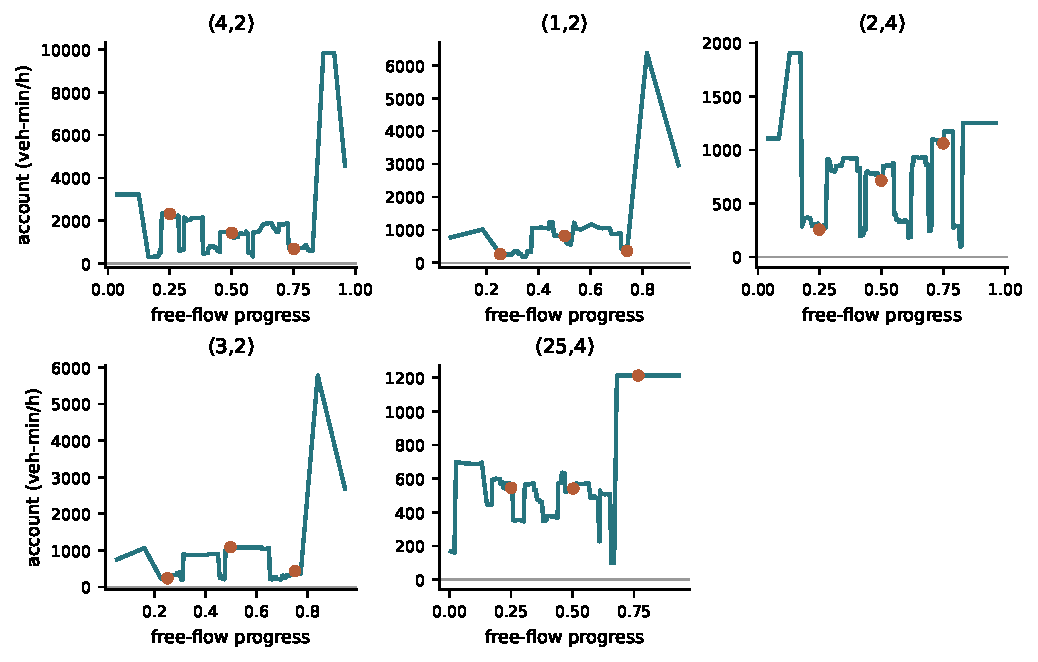
\includegraphics[width=0.99\linewidth]{../figures/fig_v106_anaheim_rest.pdf}
\caption{Anaheim spatial response profiles of the remaining five study
queries over the distance-based families: the account versus free-flow
progress along each query's own OD direction, with ochre dots marking
the three prespecified positions. All stay positive; family ranges span
roughly one to one and a half orders of magnitude.}\label{fig:anaheimrest}
\end{figure}

\subsection{Learning objectives and exact endpoint targets}\label{app:learning-objectives}
Equation~\eqref{eq:localboundarybound} suggests learning the reference's weighted demand response
where it affects spatial accounts. With training-only positive scales
$a_j$, the boundary term is
\begin{equation}
\mathcal L=\mathcal L_{\mathrm{flow}}+\lambda_J\mathcal L_{\mathrm{response}}
+\lambda_{\mathrm{cut}}\mathcal L_{\mathrm{boundary}},\qquad
\mathcal L_{\mathrm{boundary}}
=\frac1{NK}\sum_{q,j}\left[\frac{\mathcal K_j(h_j(q))}{a_j}\right]^2.
\label{eq:trainingobjective}
\end{equation}
The reference Jacobian is obtained from the existing implicit SUE
sensitivity system (Appendix~\ref{supp:sue}). We compare ordinary
flow supervision, flow plus response supervision, and the full objective.
Derivative supervision itself is established in Sobolev training
\citep{czarnecki2017sobolev}, including finite-difference derivative targets
\citep{yuan2022sobolev}; the network-derived target here selects the
part of weighted response error that changes boundary accounts.
A circulation in $\ker B$ is invisible to $\mathcal K_j$, so flow and
response losses remain necessary for the other attribution objectives.
The target matches the reference's actual response; it does not force
its true internal attribution divergence to zero or replace TSTT weights
with uniform weights. Equation~\eqref{eq:localboundarybound} is a path
inequality; finite training-point losses alone do not certify an entire
demand domain.


For the following finite-change statement, the outcome is explicitly separable:
\[
g(F)=(g_e(F_e))_{e\in E},\qquad T(F)=\sum_{e\in E}g_e(F_e).
\]
\begin{proposition}[exact finite-change boundary target]\label{prop:pairboundary}
Let $f^L,f^S$ and the edgewise outcome $g$ be continuously differentiable
on an open demand domain, and let $q^\pm=q\pm h e_j$ with their entire
segment in that domain. Put
\[
z_j^r=g(f^r(q^+))-g(f^r(q^-)),\qquad r\in\{L,S\}.
\]
For the attribution of this single-OD change,
\begin{equation}
\max_{U:s_j\in U,\ t_j\notin U}|\phi_j^L(U)-\phi_j^S(U)|
=\mathcal K_j(z_j^L-z_j^S).\label{eq:pairboundaryexact}
\end{equation}
If all sufficiently small single-coordinate changes have matching
accounts on every separating boundary at every point of the domain,
then $BD^LJ_j^L=BD^SJ_j^S$ throughout the domain. Integrating yields
matching boundary attribution columns for any joint demand path in that
domain (with the same columnwise path convention).
\end{proposition}
Appendix~\ref{app:pairproof} proves both statements. The first is an
exact finite-change target, whereas the pointwise response objective
optimizes the upper bound in Eq.~\eqref{eq:localboundarybound}; integrating
before taking $\mathcal K_j$ can retain cancellations. The second statement
requires a domain-wide local premise and is not a guarantee from finite
training data. With several ODs changing, the endpoint outcome difference
only identifies the sum of their attribution columns.

For sampled single-OD endpoint pairs, a direct training objective is
\begin{equation}
\mathcal L_{\mathrm{pair}}=\mathcal L_{\mathrm{flow}}
+\lambda_{\mathrm{edge}}\frac1N\sum_{(q,h,j)}
\frac{\|z_j^L-z_j^S\|_2^2}{b_j^2}
+\lambda_{\mathrm{cut}}\frac1N\sum_{(q,h,j)}
\left[\frac{\mathcal K_j(z_j^L-z_j^S)}{a_j}\right]^2,
\label{eq:pairobjective}
\end{equation}
with positive training-only scales $a_j,b_j$. The edge term controls
changes invisible to the boundary seminorm, whose kernel is $\ker B$.
Two reference endpoint equilibria supply $z_j^S$; training uses ordinary
parameter backpropagation through two predictions, without reference
Jacobian labels or input-Jacobian differentiation. Actual label-generation
and training costs must still be measured.

\subsection{Learned-model evaluation protocol}\label{app:pairs-v102}
Four objectives continue each of five common conservative models for 1,200 Adam
updates, with learning rate $3\times10^{-5}$, flow batch 32 and query batch eight.
The flow data and seed-specific minibatch sequences are shared. Each of six
queries has 64 training and 16 validation endpoint pairs. Centers are sampled
coordinatewise from $[0.65,1.3]$ times baseline demand (seed 102111);
half-widths 2.5\% and 15\% occur equally often. Only one demand changes per
pair, while background routes remain responsive. Endpoint-edge and
endpoint-edge-plus-boundary objectives use identical endpoint labels, coefficients
one and 0.01, and training-only root-mean-square scales. Response supervision
uses derivatives at the same pair centers; its coefficient is one.

The flow loss averages $[(f_e^L-F_e^S)/s_e]^2$ over minibatch states and edges, with $s_e=0.01\sqrt{\operatorname{mean}_{\rm train}[(F_e^S)^2]}$ from the 2,500 training states. The response loss is the batch mean of $\|J_j^L-J_j^S\|_2^2/u_j^2$. With $\langle\cdot\rangle_j$ denoting the average over query $j$'s training pair centers or endpoint labels, the scales are
\[
\begin{aligned}
u_j&=\max\{\sqrt{\langle\|J_j^S\|_2^2\rangle_j},10^{-6}\},\\
b_j&=\max\{\sqrt{\langle\|z_j^S\|_2^2\rangle_j},10^{-6}\},\qquad
a_j=\max\{\sqrt{\langle\mathcal K_j(z_j^S)^2\rangle_j},10^{-6}\}.
\end{aligned}
\]
Edge and response losses sum squared errors over edges before batch averaging; their coefficients are one, while the boundary coefficient is 0.01.

Candidates comprise the common initial model (update zero) and every 100th
continuation update. We minimize normalized validation boundary mean-square
error among candidates with mean endpoint flow error at most 1.1 times the
initial model's value, using the same 96 validation pairs for every method.
The initial model ensures this set is nonempty. Test paths never enter selection.

The 24 fixed test paths (seed 102112) contain six each with one, two, three and
six active queries; cyclic combinations balance query participation. Changes
are 15--30\% of baseline demand with both same-direction and mixed-direction
paths, each with 41 states. For every path, flow error first averages relative
Euclidean errors across its states. Attribution statistics average active
queries and seeds within each path and then take medians across the 24 paths;
seeds do not add independent paths. For column error $e_j$ and reference column
$c_j$, relative column, system and unrestricted-boundary errors divide
$\|e_j\|_2$, $|\mathbf1^\top e_j|$ and $\mathcal K_j(e_j)$ by the
corresponding reference values, with absolute floor $10^{-6}$. Geometric error
uses $\max_{U\in\mathcal F_j^{\rm geo}}|\mathbf1_U^\top Be_j|$ and
the same maximum for $c_j$. Percentages multiply ratios by 100.

The decomposition in Eq.~\eqref{eq:coldecomp} is evaluated at the same 41 states
with the same quadrature. Component norms describe error mechanisms; cancellation
prevents treating their norms as additive shares. The fixed-screenline sign
comparison in Appendix~\ref{supp:screenlinelearned} uses the separate frozen
six-query baseline segment and is not pooled with these 24 paths.
\begin{table}[t]\centering\small
\caption{The paper's principal learning comparison: four objectives with update zero included in validation selection. All prediction and explanation entries use the same 24 paths and report path medians after averaging seeds and active queries.}
\label{tab:pairs-v102}
\begin{tabular}{lrrrrr}\toprule Method & Flow (\%) & Column (\%) & System (\%) & Boundary (\%) & Geometric (\%)\\\midrule
Flow & 0.0325 & 21.61 & 2.33 & 14.53 & 7.91\\
Flow + endpoint edge & 0.0376 & 21.80 & 2.92 & 18.91 & 8.30\\
Flow + endpoint edge + boundary & 0.0376 & 21.81 & 2.95 & 18.93 & 8.30\\
Flow + response & 0.0291 & 14.22 & 3.31 & 12.08 & 5.81\\
\bottomrule\end{tabular}\end{table}
Selected updates in seed order 0--4 are Flow: 1100, 800, 1000, 100, 700; Flow + endpoint edge: 0, 1200, 0, 0, 1100; Flow + endpoint edge + boundary: 0, 1200, 0, 0, 1100; Flow + response: 1100, 1200, 1200, 1200, 1200. All selected models meet the endpoint flow constraint. For each endpoint objective, three seeds retain update zero.
On the original held-out demand-state split, seed-mean relative flow errors are Flow: 0.0386\%, Flow + endpoint edge: 0.0445\%, Flow + endpoint edge + boundary: 0.0445\%, Flow + response: 0.0388\%. These are distinct from the matched-path flow errors in the table.

\begin{table}[t]\centering\small
\caption{Incremental computation costs (seconds). Training-label and common-validation costs are measured separately on the same CPU protocol; training times are archived continuation medians, and explanation times are newly measured sequential medians for the selected models.}
\label{tab:learning-costs}
\begin{tabular}{lrrrr}\toprule Method & Training labels & Common validation & Continuation & Explanation\\\midrule
Flow & 0.00 & 6.45 & 246.0 & 7.34\\
Flow + endpoint edge & 25.75 & 6.45 & 422.2 & 7.59\\
Flow + endpoint edge + boundary & 25.75 & 6.45 & 275.1 & 7.27\\
Flow + response & 16.12 & 6.45 & 297.1 & 7.13\\
\bottomrule\end{tabular}\end{table}
Training labels comprise 768 endpoint states for either endpoint objective, or 384 center states and their sensitivities for response supervision. Every method additionally uses the same 192 endpoint states for validation; unused center-validation derivatives are excluded. Endpoint objectives share their labels and do not incur duplicate reference solves. Existing flow data, pretrained models and the common test reference are excluded from these incremental costs. The 984 test states and sensitivities took 74.4\,s in the archived reference run. Explanation timing covers all 24 paths, forward evaluation, six directional derivatives per state, quadrature and node aggregation, excluding model loading. Archived continuation times include initialization, validation and saving under concurrent seed jobs; they describe the actual training expense and do not establish a method speed advantage.


Across the five selected seeds, the ranges of mean unrestricted-boundary errors are $[13.36,24.12]\%$, $[12.29,30.50]\%$, $[12.27,30.50]\%$, $[10.53,17.46]\%$, respectively, in the method order of Table~\ref{tab:pairs-v102}. Each seed statistic first averages active queries within each path and then gives equal weight to the 24 paths. These ranges describe seed variability rather than additional independent test paths.


\section{Numerical accuracy and supporting results}\label{supp:numdetail}\label{supp:transrecords}
\subsection{Grid refinement, derivative, and solver checks}\label{supp:accuracy}
All differences here are observed numerical comparisons, not certified
bounds. Direct attribution-column differences are at most 0.178\% for
11 versus 41 states and $1.1\times10^{-4}\%$ for six-query/single-OD
41 versus 81 states. Near-zero accounts on 41/81/161 grids change by
less than $5\times10^{-6}$ percentage points (absolute $<0.01$); the
learned 201/801-state relative difference is $4.97\times10^{-6}$.
Implicit versus re-solved central-difference Jacobian errors are at most
$7.6\times10^{-5}$ (halved step $2.5\times10^{-5}$), or
$3.0\times10^{-8}$ for six-query/single-OD columns. Newton versus
successive-averages differences over 1,353 solves are at most
$1.31\times10^{-11}$. Maximum fixed-point and balance residuals are
$3.10\times10^{-8}$ and $1.82\times10^{-11}$ veh/h. Scalar completeness
relative discrepancies are at most $3.36\times10^{-5}$ for
frozen/re-routing settings and $1.9\times10^{-7}$ for single-OD checks.
Per-edge endpoint checks give relative column errors
$7.7\times10^{-8}$--$1.1\times10^{-6}$ and maximum entry residuals
$5.4\times10^{-4}$--$1.6\times10^{-2}$ TSTT units. Per-query records
remain in the arrays. The direct $(10,16)$ account change is 24.80\%
on its 41-state grid; Figure~\ref{fig:respfield} uses the seed-zero
learned model on 201 states (24.8\%).

\begin{figure}[htbp]
\centering
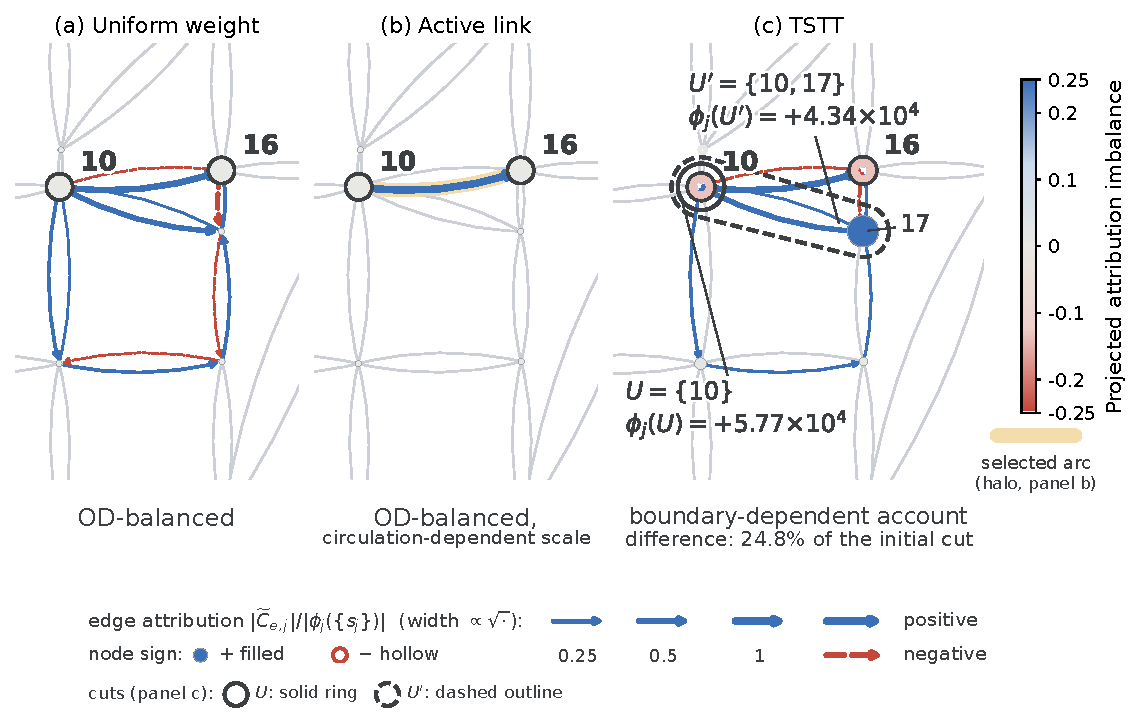
\includegraphics[width=0.84\linewidth]{../figures/fig_resp_field_v100.pdf}
\caption{OD $(10,16)$ endpoint attributions, zero background, learned
seed $0$. (a) Uniform weights give cut consistency. (b) The active-link
outcome balances in the OD direction but has no response-independent scale.
(c) The signed TSTT boundary account decreases by $24.8\%$ when the
boundary expands from $\{10\}$ to $\{10,17\}$.
Widths encode attribution magnitude; node colors show the projected
attribution imbalance $(d_j)_v$ (Eq.~\eqref{eq:endpointd}) divided by
the absolute origin-cut value.}
\label{fig:respfield}
\end{figure}

\subsection{Normalization, cancellation, and sensitivity}\label{supp:additional}
\paragraph{Complete cut-range table.}
Table~\ref{tab:cutspreadfull} completes the three representative rows of
Table~\ref{tab:cutspreadperod} with all eight study ODs.
\begin{table}[pos=htbp]
\caption{TSTT cut ranges as percentages of each account's absolute
origin-cut value, all eight study ODs (complete version of
Table~\ref{tab:cutspreadperod}). A: zero background; B: frozen background
flows; C: background demands fixed, all traffic re-equilibrated. Learned
values are five-seed medians (ranges); all SUE columns are direct
($41$ quadrature points, implicit sensitivities).}\label{tab:cutspreadfull}
\footnotesize
\begin{tabular*}{\tblwidth}{@{\extracolsep{\fill}}lccccc}
\toprule
& \multicolumn{4}{c}{Unrestricted range (\%)} & Connected (\%)\\
\cmidrule(lr){2-5}\cmidrule(lr){6-6}
OD & Learned A & SUE A & SUE B & SUE C & SUE C\\
\midrule
$(17,10)$ & $59.71$ $(58.92$--$61.23)$ & $59.95$ & $56.38$ & $54.77$ & $35.27$ \\
$(10,17)$ & $37.55$ $(37.40$--$37.94)$ & $37.48$ & $43.62$ & $49.11$ & $31.57$ \\
$(16,10)$ & $36.80$ $(36.41$--$38.40)$ & $36.86$ & $39.99$ & $166.26$ & $127.72$ \\
$(10,16)$ & $26.85$ $(26.68$--$27.07)$ & $26.94$ & $34.02$ & $109.04$ & $83.80$ \\
$(15,10)$ & $0.84$ $(0.69$--$1.16)$ & $0.77$ & $21.98$ & $84.05$ & $58.24$ \\
$(10,15)$ & $0.81$ $(0.76$--$0.88)$ & $0.77$ & $18.89$ & $71.88$ & $49.90$ \\
$(10,11)$ & $0.23$ $(0.10$--$0.35)$ & $0.0075$ & $1.17$ & $84.67$ & $51.27$ \\
$(11,10)$ & $0.18$ $(0.03$--$0.27)$ & $0.0073$ & $0.79$ & $81.09$ & $48.98$ \\
\bottomrule
\end{tabular*}
\end{table}
\paragraph{Error-metric definitions.}
The surrogate test flow error is, within each seed, the mean over the
$857$ test demands of
$\|f(q)-F^{\mathrm{SUE}}(q)\|_2/\|F^{\mathrm{SUE}}(q)\|_2$, reported
as the median over the five seeds; Jacobian column errors
$\|J_j^{\mathrm{learned}}-J_j^{\mathrm{SUE}}\|_2/\|J_j^{\mathrm{SUE}}\|_2$
are pooled over the $5\times41\times8$ seed--point--OD columns;
attribution-column errors use the per-column norm over the $40$
seed--OD columns on the common $41$-point grid.

\paragraph{Same-path flow, sensitivity, and boundary-account errors.}
The test-split flow error is not paired with the Jacobian
comparison; re-summarized on the same $41$ zero-background quadrature
points for each seed (median / 95th percentile / maximum, percent):
flow error $0.136$ / $0.682$ / $1.331$; Jacobian column error
$0.516$ / $3.903$ / $9.562$ (maximum at seed $3$, OD $(16,10)$,
$\lambda=0.925$; $5\times41\times8$ seed--point--OD units);
attribution-column
errors median $0.349\%$, maximum $1.80\%$; and
$E_j^{\mathrm{cut}}$, which evaluates both models' accounts at every
connected boundary of a query's family on the same path
(the unrestricted-family counterpart is virtually identical), at
$0.204$ / $0.650$ / $1.739$ ($40$ seed--OD units; largest connected
error at OD $(16,10)$, seed $3$).

Table~\ref{tab:origin_denominators} supplies the per-query absolute
origin-cut denominators for Table~\ref{tab:cutspreadperod}. The
setting-C link sums $C_j$ span $2.078$--$4.282\times10^5$ TSTT units,
exceeding origin-cut accounts by factors of $1.01$--$2.37$; their sum
matches the endpoint TSTT change within $2.3\times10^{-5}$ relative.
\begin{table}[pos=htbp]
\caption{Absolute direct-SUE origin-cut accounts
$|\phi_j(\{s_j\})|$, in TSTT units, for the eight queries in
Table~\ref{tab:cutspreadperod}. A, B, C use their respective
$41$-point columns; entries rounded to one decimal.}
\label{tab:origin_denominators}
\footnotesize
\begin{tabular*}{\tblwidth}{@{\extracolsep{\fill}}lrrr}
\toprule
OD & A & B & C\\
\midrule
$(17,10)$ & $29{,}372.1$ & $249{,}729.2$ & $224{,}954.3$ \\
$(10,17)$ & $46{,}977.2$ & $317{,}861.9$ & $245{,}178.7$ \\
$(16,10)$ & $41{,}994.3$ & $352{,}858.5$ & $180{,}671.5$ \\
$(10,16)$ & $57{,}468.9$ & $405{,}374.2$ & $272{,}743.2$ \\
$(15,10)$ & $33{,}859.4$ & $226{,}878.2$ & $201{,}351.2$ \\
$(10,15)$ & $34{,}056.4$ & $258{,}682.3$ & $232{,}160.6$ \\
$(10,11)$ & $28{,}807.1$ & $339{,}651.4$ & $202{,}928.2$ \\
$(11,10)$ & $28{,}010.4$ & $324{,}427.0$ & $204{,}802.3$ \\
\bottomrule
\end{tabular*}
\end{table}

The node breakdown in Table~\ref{tab:bgdecomp} complements the fixed
boundary comparison of Section~\ref{subsec:bgsplit}.
\begin{table}[pos=htbp]
\caption{Signed node divergence in the re-routing setting, at the
same joint equilibrium state and total-flow gradient at each of the
$41$ quadrature points (study includes all eight query ODs; TSTT
units of Appendix~\ref{supp:networks}; entries rounded independently,
so a component sum may differ from the rounded total in its last
digit).}
\label{tab:bgdecomp}
\small
\begin{tabular*}{\tblwidth}{@{\extracolsep{\fill}}llrrr}
\toprule
OD & Node & Study & Background & Total\\
\midrule
$(10,16)$ & $15$ & $-973.1$ & $49,103.4$ & $48,130.3$ \\
$(10,16)$ & $8$ & $9.6$ & $42,102.7$ & $42,112.3$ \\
$(10,16)$ & $20$ & $0.2$ & $41,805.4$ & $41,805.6$ \\
$(10,11)$ & $5$ & $0.5$ & $35,952.1$ & $35,952.6$ \\
$(10,11)$ & $12$ & $0.0$ & $-23,858.1$ & $-23,858.1$ \\
$(10,11)$ & $9$ & $-0.2$ & $-18,557.6$ & $-18,557.7$ \\
\bottomrule
\end{tabular*}
\end{table}

For the learned zero-background low-range group, five-seed median pointwise
imbalance budgets $100A_j/|\phi_j(\{s_j\})|$ lie between $0.22\%$ and
$0.95\%$, versus $26.85$--$59.71\%$ for the high group; the low-group
median cancellation factors are at most $0.313$ (one seed reaches
$\kappa=0.852$), so small pointwise imbalance mainly limits the
low-group range, while the high group's median $\kappa$ is below
$8\times10^{-5}$.

Zero-background route-choice dispersion checks at $\theta\in\{0.5,1,2\}$
(eleven-point direct-SUE calculations) retain the large/small
separation --- large ranges $27$--$64\%$, the others below $9.4\%$.

\subsection{Full-background six-query surrogate validation}\label{supp:fullbgsurrogate}
The six-query conservative surrogate predicts shares over all 5,280
paths, with the architecture of Appendix~\ref{supp:protocol}, dataset
seed 20261025 and batch size 256. Its 4,214 target solves have maximum
path residual $3.5\times10^{-8}$; learned conservation residual is at
most $3.6\times10^{-11}$. Held-out flow error is 0.040\% (seed median;
range 0.035--0.056\%). On the 41 common path states, flow errors are
0.037--0.065\%, but increment errors are 5.0--7.0\% against a reference
increment norm 2,982.7 (2.7\% of flow level). Median column errors are
81.2\% for $(7,18)$, 31.1\% for $(4,5)$ and 7.4--11.8\% for the
others. System contribution errors reach 14.7\% and 10.3\% for those
two queries, versus at most 3.7\% for the sign-crossing queries.
Table~\ref{tab:fullbgsurrogate} retains extrema and boundary errors;
learned column completeness is within $6\times10^{-6}$ relative.

An exact two-term split of \eqref{eq:Cdef} ($L$/$S$: learned/direct)
identifies where this error arises:
\begin{equation}
\widetilde C_{:,j}^{L}-\widetilde C_{:,j}^{S}
=\Delta q_j\int_0^1(D_\lambda^{L}-D_\lambda^{S})J_j^{S}\,\mathrm{d}\lambda
+\Delta q_j\int_0^1D_\lambda^{L}(J_j^{L}-J_j^{S})\,\mathrm{d}\lambda,
\label{eq:coldecomp}
\end{equation}
satisfied entrywise within $10^{-10}$ TSTT units. The weight-shift
term has querywise median norm at most 0.2\% of the reference column;
the response term is larger in every one of the thirty seed--query
units. Their norm sum is at most 1.04 times the realized error norm.
Signed scalar terms can cancel, so these norms are not additive shares.
Small-band endpoint columns have 4.8--15.9\% error and system values
within 2.7\% of reference, while every seed retains the reported signs.

\subsection{Sensitivity to candidate paths and route-choice dispersion}\label{supp:coverage}
The path-set comparison expands all $528$ OD sets to twenty
candidates each (the first ten unchanged), with demands, BPR
functions, $\theta=1$, and $41$ quadrature points fixed: across the
eight queries, absolute unrestricted and connected ranges change by
at most $0.977\%$ and $1.011\%$, with the three largest
internal-node terms keeping their ordered node IDs (moving at most
$1.43\%$). The $\theta\in\{0.5,2\}$ check splits the specified
$(10,16)$ boundary difference into study/background components
$-7{,}404.9$/$-2{,}371.5$ at $\theta=0.5$ and $+115.3$/$+235.7$ at
$\theta=2$; for all three additional models, implicit derivative
columns match re-solved half-step central differences at the
demand-path midpoint (maximum $0.00249\%$, completeness gap
$2.85\times10^{-5}$).

\subsection{Six-query interval, mechanism, boundary-family, and
scenario checks}\label{supp:newodaccuracy}


\textbf{Extremal ranges and negative shares.}
Unrestricted extrema follow the closed form \eqref{eq:cutextrema},
connected extrema the same enumeration as the connected ranges
(Table~\ref{tab:newodinterval}); the negative shares in
Section~\ref{subsec:newod} are exact counts over the connected
families ($4{,}621$--$16{,}943$ admissible sets per query), and all
displayed values come from the $41$-point columns.

\begin{table}[pos=tbh]
\caption{Minimum--maximum boundary-account ranges for the three
sign-crossing queries of Table~\ref{tab:newod}, in TSTT units
(Appendix~\ref{supp:networks}), rounded to integers. Baseline:
unrestricted extrema (closed form \eqref{eq:cutextrema}; connected
extrema in Table~\ref{tab:newod}); next four rows: connected
ranges under the model-setting changes and the single-OD
$0.2\to1.6$ re-run (unrestricted intervals within $1\%$ of the
baseline row); last two: small-interval bands, with $C_j$ positive
($+7{,}202$ to $+33{,}734$ across the three queries) and the control
$(6,8)$ positive ($[5{,}079,\ 9{,}623]$ and $[10{,}157,\ 19{,}246]$;
single-OD $[35{,}352,\ 66{,}861]$).}
\label{tab:newodinterval}
\footnotesize
\begin{tabular*}{\tblwidth}{@{\extracolsep{\fill}}lrrr}
\toprule
Range & $(1,19)$ & $(1,15)$ & $(7,12)$\\
\midrule
Baseline ($10$ paths, $\theta=1$): unrestricted & $[-19{,}116,\ 26{,}696]$ & $[-16{,}240,\ 44{,}137]$ & $[-45{,}241,\ 61{,}650]$\\
\addlinespace
Twenty paths, $\theta=1$: connected & $[-13{,}451,\ 24{,}276]$ & $[-8{,}329,\ 40{,}644]$ & $[-17{,}728,\ 59{,}452]$\\
Ten paths, $\theta=0.5$: connected & $[-13{,}024,\ 24{,}064]$ & $[-8{,}107,\ 39{,}933]$ & $[-17{,}633,\ 60{,}476]$\\
Ten paths, $\theta=2$: connected & $[-13{,}016,\ 24{,}411]$ & $[-8{,}233,\ 40{,}892]$ & $[-19{,}587,\ 61{,}647]$\\
Single-OD $0.2\to1.6$: connected & $[-13{,}608,\ 24{,}414]$ & $[-8{,}359,\ 40{,}745]$ & $[-17{,}580,\ 60{,}006]$\\
Single-OD $\pm10\%$ band ($0.9\to1.1$): connected & $[-1{,}947,\ 3{,}494]$ & $[-1{,}201,\ 5{,}838]$ & $[-2{,}517,\ 8{,}608]$\\
Single-OD $\pm20\%$ band ($0.8\to1.2$): connected & $[-3{,}895,\ 6{,}988]$ & $[-2{,}402,\ 11{,}677]$ & $[-5{,}035,\ 17{,}215]$\\
\bottomrule
\end{tabular*}
\end{table}

\textbf{Connected minimum and divergence decomposition.}
Table~\ref{tab:negmech} reports, for each sign-crossing query, the
connected minimizing boundary $U_-$ at the baseline setting: its
account, and the interior divergence sum
$\phi_j(\{s_j\})-\phi_j(U_-)$, decomposed as the table caption
specifies, at the same joint state and gradient as the reported
columns (additivity $\le1.2\times10^{-10}$).
By Eq.~\eqref{eq:cutgap}, the negative divergence captured inside
$U_-$ ($4{,}664.9$, $6{,}960.1$, and $19{,}811.5$ for the three
queries) covers $83\%$, $88\%$, and $72\%$ of the gaps
$\phi_j(U_-)-\phi_j^{\min}$, while the captured positive divergence
($19{,}938.0$, $18{,}194.2$, $46{,}901.4$) is $95.5\%$, $94.8\%$,
and $85.7\%$ of the query totals. The sign change arises
differently across queries: study response
dominates for $(1,19)$ (largest node $15$: own $+14{,}464.0$),
study- and background-dominated nodes share the sign for $(1,15)$,
and both contribute about equally for $(7,12)$ (node $8$).
The extremal node sets (one-based node IDs) are
$U_-(1,19)=\{1,2,6,7,8,9,15,16,18,20,21,22,24\}$ and
$U_+(1,19)=\{1,2,3,4,5,6,10,11,12,13,14,22,23\}$;
$U_-(1,15)=\{1,2,6,7,8,9,16,17,18,19,20,21,24\}$ and
$U_+(1,15)=\{1,2,3,4,5,6,10,11,12,13,14,22,23\}$;
$U_-(7,12)=\{1,2,3,4,5,6,7,8,9,10,11,14,17,19,23\}$ and
$U_+(7,12)=\{7,8,9,15,16,18,20,21,22,24\}$.

\begin{table}[pos=tbh]
\caption{Connected minimizing boundary $U_-$ at the baseline setting
for the three sign-crossing queries, in TSTT units. Interior is the
divergence sum over $U_-\setminus\{s_j\}$, decomposed into the query's
own response, the other five query ODs, and the background response;
the study group of the main text is the sum of the first two columns.
Node sets are the one-based lists in the preceding paragraph. Entries
are rounded independently.}
\label{tab:negmech}
\small
\begin{tabular*}{\tblwidth}{@{\extracolsep{\fill}}lrrrrrr}
\toprule
OD & $\phi_j(\{s_j\})$ & $\phi_j(U_-)$ & Interior & Own OD & Other query & Background\\
\midrule
$(1,19)$ & $1{,}771.6$ & $-13{,}501.6$ & $15{,}273.1$ & $19{,}480.9$ & $-59.4$ & $-4{,}148.3$ \\
$(1,15)$ & $2{,}948.1$ & $-8{,}286.0$ & $11{,}234.1$ & $7{,}856.9$ & $-26.7$ & $3{,}404.0$ \\
$(7,12)$ & $9{,}473.8$ & $-17{,}616.2$ & $27{,}089.9$ & $14{,}002.3$ & $-3.2$ & $13{,}090.8$ \\
\bottomrule
\end{tabular*}
\end{table}

\textbf{Neighbourhood families.}
Use undirected hop distance or shortest free-flow distance from the origin
(minimum weight over parallel arcs). Include nodes at each attained radius,
stop before including the destination, and retain only two-sided connected
regions. Table~\ref{tab:neighbourhoods} reports all family ranges; all are
positive with minima at the origin cut. For short-path queries $(7,18)$,
$(4,5)$ and $(6,8)$, only that cut is admissible. The thirteen-node
free-flow ball at radius 16 for $(1,19)$ is
$\{1,2,3,4,5,6,7,8,9,11,12,13,24\}$, with account $+10{,}756.0$.

\begin{table}[pos=htbp]
\caption{Origin-centred neighbourhood accounts, baseline six-query setting C
(TSTT units). Counts are distinct admissible node sets within each family;
sets shared by the two families are counted in each row.}\label{tab:neighbourhoods}
\footnotesize
\begin{tabular*}{\tblwidth}{@{\extracolsep{\fill}}llrrr}
\toprule OD & Neighbourhood & Count & Minimum & Maximum\\\midrule
$(1,19)$ & Hop distance & 6 & $1,771.6$ & $15,803.5$\\
$(1,19)$ & Free-flow time & 13 & $1,771.6$ & $15,803.5$\\
$(1,15)$ & Hop distance & 5 & $2,948.1$ & $26,602.0$\\
$(1,15)$ & Free-flow time & 14 & $2,948.1$ & $26,602.0$\\
$(7,12)$ & Hop distance & 4 & $9,473.8$ & $31,524.1$\\
$(7,12)$ & Free-flow time & 9 & $9,473.8$ & $32,139.4$\\
\bottomrule\end{tabular*}\end{table}

\textbf{Straight screenlines.}
Coordinates use an equirectangular frame (longitude scaled by the cosine
of mean latitude). Section~\ref{sec:scan}'s 36-direction construction,
with duplicate regions removed, gives 35, 152, 32, 123, 23 and 148
regions in Table~\ref{tab:newod} order. All accounts agree with direct
incidence aggregation below $10^{-9}$. Refining directions from
$5^\circ$ to $1^\circ$ leaves both negative minima unchanged; negative
shares change from 1.3\% to 1.8\% for $(1,19)$ and 6.8\% to 6.2\%
for $(7,12)$. Other queries stay positive; only $(7,18)$'s minimum
changes, from 642.4 to 641.4.

\textbf{Model-setting checks.}
Re-solving the protocol of Appendix~\ref{supp:newod} under twenty
candidate paths per OD and $\theta\in\{0.5,2\}$ at ten paths gives
the ranges of Table~\ref{tab:newodinterval} ($C_j$ within $3.9\%$);
solver and finite-difference checks match
Appendix~\ref{supp:newod} levels.

\textbf{Single-OD demand changes.}
Each single-OD demand path ($0.2\to1.6$ of published demand)
re-solves the setting-C protocol with one moving coordinate. For the
three crossing queries the connected ranges (Table~\ref{tab:newodinterval},
single-OD row) still straddle zero, their extrema attained by exactly
the joint-scenario sets $U_-$ and $U_+$ (changes at most $0.9\%$ and
$0.5\%$; unrestricted intervals within $1\%$ of the joint baseline)
and the contributions stay positive ($C_j=50{,}322.2$, $77{,}672.6$,
$117{,}476.8$); the control $(6,8)$ remains sign-consistent
($C_j=74{,}176.1$, connected range in the caption). The
small-interval bands (Table~\ref{tab:newodinterval}, last two rows)
follow the same protocol, the $41$-point check ($(1,19)$,
$0.8\to1.2$) reproducing the endpoint column to $1.3\times10^{-5}$
TSTT units per edge.

\begin{figure}[pos=htbp]
\centering
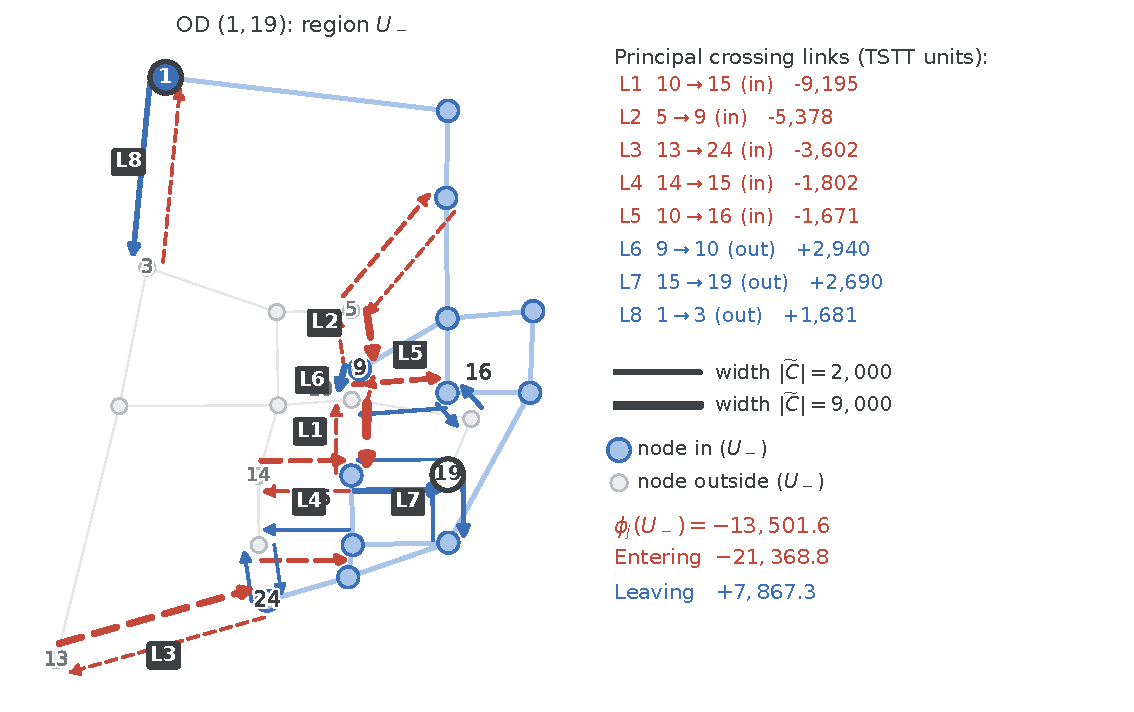
\includegraphics[width=0.82\linewidth]{../figures/fig_negmech_v102.pdf}
\caption{The connected minimizing region $U_-$ for OD $(1,19)$
(setting C, six-query protocol). Shaded nodes form $U_-$ (origin
node $1$ ringed; destination $19$ outside). Crossing-link arrows keep
the link direction; width scales with $|\widetilde C_{e,j}|$, and
colour and style encode the signed contribution to $\phi_j(U_-)$,
$a_{e,j}=\sigma_e\widetilde C_{e,j}$ ($\sigma_e=+1$ leaving, $-1$
entering; solid blue positive, dashed red negative), so a positive
attribution on an entering link appears red. The side panel lists, in
TSTT units, the five largest negative and three largest positive
contributions among the $26$ crossing links
($\mathrm{L}1$--$\mathrm{L}5$ negative, $\mathrm{L}6$--$\mathrm{L}8$
positive, ``(in)''/``(out)'' marking entering and leaving links),
with the width scale and the membership legend.}
\label{fig:negmech}
\end{figure}
\textbf{Endpoint identity checks.}
Appendix~\ref{supp:accuracy} reports the per-edge
endpoint-identity errors and their relation to completeness gaps on
these same demand paths.

\FloatBarrier
\subsection{Baseline surrogate envelopes}\label{supp:baselineenvelopes}
\begin{table}[pos=htbp]
\caption{Full-background surrogate validation on the identical
$41$-state path of the six-query protocol (setting C; TSTT units;
contributions and extrema rounded to integers, errors to one
decimal). $C_j^{\mathrm{learned}}$ and the connected extrema:
across-seed envelopes of per-model values (direct-SUE values in
Table~\ref{tab:newod}). Last two columns: five-seed
\emph{median} of the largest connected-boundary disagreement
$\epsilon_j^{\mathrm{cut}}$, in absolute units and as a percentage of
the direct connected span.}
\label{tab:fullbgsurrogate}
\footnotesize
\begin{tabular*}{\tblwidth}{@{\extracolsep{\fill}}lrrrrr}
\toprule
& & \multicolumn{2}{c}{Connected extrema: across-seed ranges}\\
\cmidrule(lr){3-4}
OD & $C_j$: across-seed envelope & per-model minima & per-model maxima & $\epsilon^{\mathrm{cut}}$ (med.) & $\epsilon^{\mathrm{cut}}$/span (med., \%)\\
\midrule
$(7,18)$ & $[574,\ 681]$ & $[335,\ 521]$ & $[907,\ 1{,}299]$ & $397.5$ & $522.5$ \\
$(1,19)$ & $[49{,}929,\ 51{,}452]$ & $[-13{,}911,\ -13{,}334]$ & $[23{,}683,\ 23{,}948]$ & $1{,}567.4$ & $4.2$ \\
$(4,5)$ & $[2{,}535,\ 2{,}934]$ & $[1{,}654,\ 2{,}148]$ & $[2{,}946,\ 3{,}546]$ & $1{,}050.8$ & $99.5$ \\
$(1,15)$ & $[77{,}416,\ 80{,}233]$ & $[-7{,}717,\ -6{,}766]$ & $[39{,}473,\ 40{,}076]$ & $2{,}187.3$ & $4.5$ \\
$(6,8)$ & $[73{,}565,\ 75{,}224]$ & $[36{,}412,\ 37{,}631]$ & $[66{,}892,\ 67{,}762]$ & $2{,}163.2$ & $6.9$ \\
$(7,12)$ & $[116{,}562,\ 118{,}706]$ & $[-17{,}084,\ -15{,}198]$ & $[59{,}965,\ 61{,}169]$ & $4{,}111.3$ & $5.3$ \\
\bottomrule
\end{tabular*}
\end{table}



\subsection{Fixed-screenline surrogate comparisons}\label{supp:screenlinelearned}
\begin{table}[pos=htbp]
\caption{Fixed straight screenlines: reference minimum and the five frozen flow-supervised surrogates at that same screenline (TSTT units). The last column gives the largest error over the screenline family, as an across-seed range.}
\label{tab:screenlinelearned}
\small\begin{tabular*}{\tblwidth}{@{\extracolsep{\fill}}lrrr}\toprule
OD & Reference minimum & Learned account: seed range & Maximum screenline error: seed range\\\midrule
$(7,18)$ & 642.4 & $[576.9,\ 789.8]$ & $[141.0,\ 269.4]$ \\
$(1,19)$ & -2766.6 & $[-3886.6,\ -3365.1]$ & $[857.9,\ 1430.8]$ \\
$(4,5)$ & 2652.3 & $[2301.7,\ 2918.8]$ & $[438.0,\ 648.3]$ \\
$(1,15)$ & 511.1 & $[732.8,\ 2068.2]$ & $[1140.6,\ 2553.0]$ \\
$(6,8)$ & 45230.2 & $[46431.5,\ 47218.3]$ & $[1276.2,\ 1988.1]$ \\
$(7,12)$ & -2967.3 & $[-2810.4,\ -1916.6]$ & $[1736.8,\ 2499.2]$ \\
\bottomrule\end{tabular*}\end{table}


\paragraph{Sign preservation.}\label{subsec:precision}
All five baseline seeds retain the three connected-family sign crossings
and positive system contributions. At the fixed reference extrema,
$m_j=\min\{-\phi_j^S(U_-),\phi_j^S(U_+)\}-\epsilon_j^{\rm conn}$
is positive, with smallest value 5519 TSTT units. This verifies sign
preservation without implying accurate column magnitudes.

At the fixed direct-model minimizing screenline, every baseline seed
retains the negative sign for both queries: $(1,19)$ gives
$[-3886.6,-3365.1]$ against the reference $-2766.6$, and $(7,12)$
gives $[-2810.4,-1916.6]$ against $-2967.3$. Their largest family-wide
errors across seeds are $1430.8$ and $2499.2$, below the respective
reference sign margins. These are screenline-specific certificates;
they supplement the separate connected-family result above
(Appendix~\ref{supp:screenlinelearned}).


The eight-query path-set and dispersion checks are collected in
Appendix~\ref{supp:coverage}. Boundary variation persists, although
the specified $(10,16)$ comparison $\{10\}\to\{10,17\}$ changes sign
across $\theta$; these are different fixed-path models, not convergence
to unrestricted SUE.

\subsection{Additional learning comparisons}\label{app:legacy-learning}\label{app:learning-protocol}\label{app:calibration-protocol}
Two additional pointwise comparisons use five conservative models, 600 Adam updates at $3\times10^{-5}$, flow/response batches of 32/8 and training-only scales. Derivative labels comprise 256 training and 64 validation states (seed 20261029). The fixed-coefficient comparison uses coefficients one; calibration selects 0.01 from $\{0.001,0.01,0.1\}$ with seed zero under a 110\% relative flow-error threshold, then applies it across seeds (seven boundary fits). Each comparison tests four prescribed 41-state paths, with one, two, three and six active queries and baselines in $[0.65,1.3]$ times published demands (test seeds 101029/101030). Fixed-coefficient boundary supervision yields 22.25\% boundary error versus 9.64\% for response supervision; calibration yields 7.74\% versus 7.44\% on its new paths. Neither comparison supports overall improvement. Complete current four-method results, with common selection and matched-path metrics, are in Table~\ref{tab:pairs-v102}.

\subsection{Complete input-stratified common-summary results}\label{sec:coverage}
Positive non-diagonal published demands are stratified by demand and directed free-flow shortest-path time using empirical tertiles, with ties kept in the lower bin. Within each of nine cells, lexicographically sorted OD indices at zero-based positions $\lfloor N/3\rfloor$ and $\lfloor2N/3\rfloor$ are retained. No attribution values enter selection. Endpoint differences identify total edge attribution, without identifying the same-state study/background response split. The two perturbation widths share every field of the selection protocol and differ only in the demand interval; their normalized errors are close for every query, so Table~\ref{tab:coveragefull} reports both in one table. Absolute minima, maxima, midpoints and half-ranges for both widths, and the per-position account sequences behind the segmentation of Proposition~\ref{prop:segmented}, accompany the result arrays in the code package.
\begin{table}[pos=htbp]\centering\footnotesize\caption{Complete geometric common summaries for the 18 input-stratified queries at both widths. Normalized error is Eq.~\eqref{eq:normerror} at $\pm10\%$ and $\pm20\%$; ranges are $[\phi_{\min},\phi_{\max}]$ at $\pm20\%$ in Sioux Falls cost units; P and M mean positive and mixed signs at $\pm20\%$.}\label{tab:coveragefull}\begin{tabular}{lrrrrl}\toprule OD & System & Range ($\pm20\%$) & Norm.\ err.\ ($\pm10\%$) & Norm.\ err.\ ($\pm20\%$) & Sign\\\midrule
(4,3) & 507.2 & [429.0, 535.0] & 9.9 & 9.9 & P\\
(12,3) & 337.2 & [330.7, 340.2] & 1.4 & 1.4 & P\\
(6,1) & 2360.6 & [658.3, 2290.4] & 35.6 & 35.6 & P\\
(15,6) & 9390.2 & [415.4, 4433.5] & 45.3 & 45.3 & P\\
(6,21) & 4577.8 & [-3.4, 2349.4] & 50.1 & 50.1 & M\\
(18,14) & 3422.3 & [150.8, 1929.7] & 46.1 & 46.1 & P\\
(8,4) & 25097.5 & [1270.7, 15741.3] & 46.0 & 46.0 & P\\
(19,8) & 16939.7 & [733.2, 7266.4] & 45.0 & 45.0 & P\\
(11,6) & 6165.9 & [1236.4, 6106.4] & 39.9 & 39.9 & P\\
(16,2) & 17763.1 & [896.3, 9628.6] & 45.3 & 45.3 & P\\
(8,21) & 7605.5 & [752.6, 4214.1] & 41.1 & 41.1 & P\\
(14,8) & 17445.3 & [890.3, 7527.1] & 44.1 & 44.1 & P\\
(11,15) & 47925.5 & [17628.9, 27737.8] & 18.2 & 18.2 & P\\
(17,9) & 24040.9 & [5482.3, 18519.3] & 35.2 & 35.2 & P\\
(10,12) & 55214.5 & [9822.4, 33248.6] & 35.2 & 35.2 & P\\
(13,10) & 54411.9 & [2918.8, 31345.2] & 45.3 & 45.3 & P\\
(1,10) & 33917.2 & [2182.9, 20856.4] & 44.8 & 44.8 & P\\
(10,1) & 34264.5 & [2182.7, 21039.5] & 44.8 & 44.8 & P\\
\bottomrule\end{tabular}\end{table}

\begin{figure}[pos=htbp]\centering
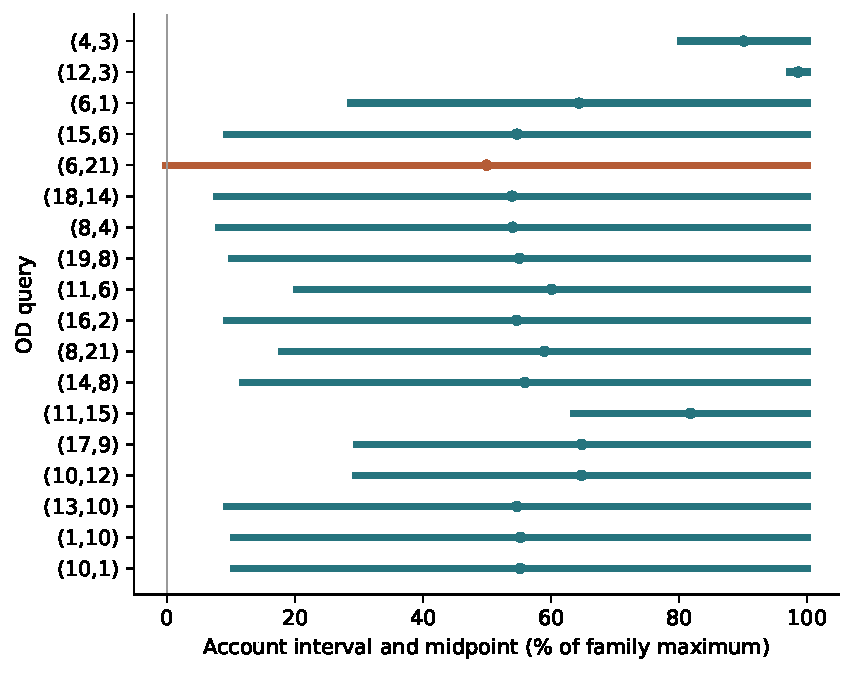
\includegraphics[width=0.88\linewidth]{../figures/fig_v106_coverage_intervals.pdf}
\caption{Geometric account intervals normalized by each query's largest
account magnitude, over all 18 input-stratified queries at $\pm20\%$
(the complete-interval companion of
Figure~\ref{fig:commonsummary}).}\label{fig:coverageintervals}
\end{figure}

